\subsection{Identifying and Moving Objects to H2}
\label{sec:api}

\teraheapName{} provides a hint-based interface, enabling frameworks to tag
root key-objects with a label for H2 movement, via a new field (eight
bytes for alignment purposes) in the Java object header.
Alternatively, we can avoid this field by using additional JVM
metadata for storing the address of each object that needs to be moved
to H2. However, this would increase \teraheapGC time because it requires
updating object accesses in every \teraheapGC cycle until they are moved to
H2. The \teraheapName{} interface consists of the following function calls.

\textbf{h2\_tag\_root(obj, label):}
The framework uses \texttt{h2\_tag\_root()} to tag a root key-object
with a label.

\textbf{h2\_move(label):}
The framework uses \texttt{h2\_move()} to advise \teraheapName{} to move all
objects with the specified label to H2. During the next major \teraheapGC, the
garbage collector identifies the root key-objects tagged with the same
label as the specified label. Then it detects and marks for moving to
H2 objects in the transitive closure of the root key-object by tagging
these objects with the same label as the root-key object.

Typically, frameworks can use \texttt{h2\_move()} once their object
group becomes immutable. However, immutability is not a strict
requirement for movement to H2 and partly depends on storage device
characteristics~\cite{swanson:nvm}. For instance, in Spark, all
objects can be moved when marking the root key-object, whereas, in
Giraph, objects are best moved at the end of each computation stage,
possibly much later than when marking the root key-object.

Delaying the move to H2 runs the danger of creating out-of-memory
errors because H1 may fill before \texttt{h2\_move()} is called.  To
avoid this, \teraheapName{} monitors the space that live objects occupy at the
end of each major \teraheapGC. If the live objects occupy more space in H1
than a high threshold (e.g., 85\% of H1), \teraheapName{} will move marked
objects to H2 during the next major \teraheapGC without waiting for
\texttt{h2\_move().}

At this point, if \teraheapName{} moves all marked objects to H2, it may incur
excessive device traffic, e.g., in case some of these objects may be
updated frequently prior to the application using \texttt{h2\_move().}
To mitigate this effect, \teraheapName{} uses a low threshold mechanism as
well, which limits how many marked objects will move to H2 when
\teraheapName{} detects high H1 pressure prior to seeing an
\texttt{h2\_move()} hint. In our evaluation, we also examine the
alternative of not using \texttt{h2\_move()} and relying only on the
high-low threshold mechanism.

Placing objects with the same label in the same H2 region allows
\teraheapName{} to reclaim them en masse. However, the transitive closure
might include specialized objects that can have a longer lifetime and
delay the region from being freed. For this reason, \teraheapName{} excludes
from the transitive closure:
%
(1) JVM metadata, such as \emph{class
objects}~\cite{ClassJav88:online} and the class loader, and
%
(2) objects that inherit the \emph{java.lang.ref.Reference}
class~\cite{Referenc77:online}.

The JVM automatically creates class objects upon class loading. Each
class has one class object containing the static fields of the class
and multiple instance objects. As all instances share the static
fields, class objects are not reclaimed until the last instance object
of the class dies, which triggers the JVM to unload the class. As a
result, class objects may be updated frequently due to static fields
and exhibit long lifetimes.

Objects that inherit from the java.lang.ref.Reference class (such as
soft, weak, final, and phantom references) require special treatment
by the garbage collector. The garbage collector maintains four lists,
one for each kind of reference. During the object graph traversal, the
garbage collector adds the discovered live objects with these reference
types to the respective lists. Then, it applies a
different collection policy for each reference type. For example, soft
references keep the objects alive as long as memory is available on
the heap but discard them before an out-of-memory error.
Thus, objects with soft, weak, final, and phantom references have different
lifetimes than those in the closure, extending the region's lifetime and
preventing free operations.

\teraheapName{} moves marked objects from H1 to H2 during major \teraheapGC. To reduce
this cost, \teraheapName{} uses explicit asynchronous I/O. We avoid multiple
system calls for small-sized objects ( <\SI{1}{MB}), using a promotion
\SI{2}{MB} buffer per region in H2 that writes objects to the device
in batches.

\subsection{Reclaiming Dead Regions}
\label{sec:free}
Figure~\ref{fig:allocator} shows the region-based organization of H2
in virtual memory and each region metadata in DRAM. Unlike
Broom~\cite{gog:broom}, we do not impose any restrictions on regions,
allowing objects in any region to refer to each other. \teraheapName{} ensures
that while reclaiming a region, none of the objects in the region are
referenced from live H1 or H2 objects in other regions. To find such
regions, \teraheapName{} tracks cross-region and forward references without
scanning H2 objects, which would generate excessive I/O.

\begin{figure}
	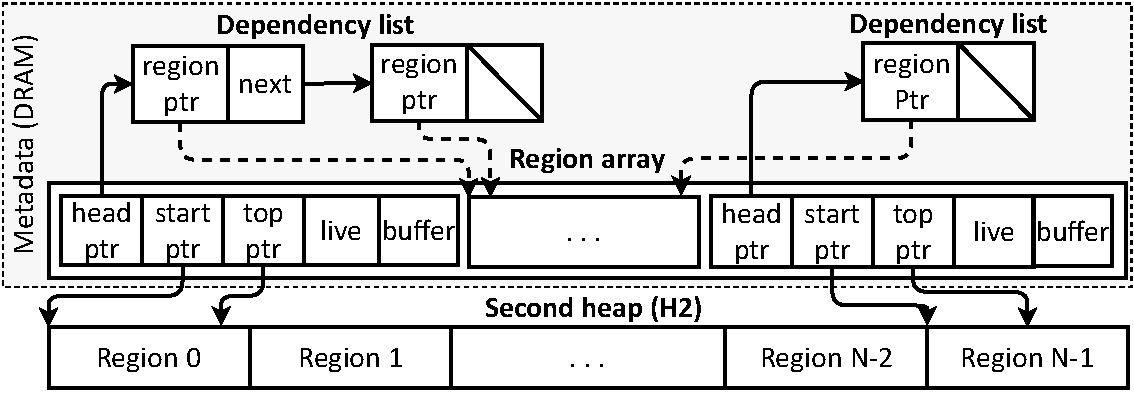
\includegraphics[width=0.6\linewidth]{teraheap/fig/allocator-crop.pdf}
	\caption{H2 allocator metadata in DRAM.}
	\label{fig:allocator}
\end{figure}

\paragraph{\textbf{Cross-region references in H2}}
To allow internal H2 references \emph{across} regions, \teraheapName{} tracks
the direction of cross-region references. As shown in
Figure~\ref{fig:allocator}, \teraheapName{} keeps a dependency list in
per-region metadata in DRAM. Each node of the dependency list points
to a (different) region referenced by objects of the current region.
When we move objects to H2 we check if they have references in
existing H2 regions. Then, the H2 allocator adds a new node (if it
does not exist) to the dependency list of the region where objects
will be moved.
Another case we must consider is when an object in an existing H2
region (e.g., region A) references a candidate object in H1 that will
be moved to a different region (e.g., region B) in H2. In this case,
we update the dependency list of region A while updating the backward
references from objects in H2 to objects in H1.
The size of dependency lists is small, on average 10
nodes per region in our evaluation.

We also explore a simpler, \emph{Union-Find} approach, using the
notion of region groups that avoids tracking the direction of
cross-region references. We track cross-region references by logically
merging the source and destination regions in a single region group.
Region groups grow over time to include all regions with cross-region
references. If there is any reference from H1 to any object in the
group's regions, then we consider the group alive. This approach does
not consider the direction of region references, missing opportunities
to reclaim dead regions with no incoming references. For instance, if
there is a reference from region X to Y and a reference from region Y
to Z, all three regions belong to the same region group and can be
reclaimed when the whole group dies. We find that the direction of
references matters for more efficient space reclamation. In the
previous example, if only region Z is referenced by H1, then regions X
and Y can still be reclaimed.

\paragraph{\textbf{Forward references (H1 to H2)}}
\teraheapName{} avoids scanning H2 objects by fencing the garbage collector
from crossing into H2 from H1. This requires identifying all
references from H1 to H2 and marking the referenced H2 objects as
alive. \teraheapName{} uses a \texttt{live} bit in the per-region metadata
(Figure~\ref{fig:allocator}) that signifies the objects in the region
are reachable from H1. The garbage collector clears \texttt{live} bits at the
beginning of the major \teraheapGC. Upon encountering a reference from an
object in H1 to an object in H2, the collector sets the corresponding
region bit. If the dependency list of the current region is not empty,
then we traverse the dependency lists of each dependent region
recursively, setting their \texttt{live} bits, as well.

\paragraph{\textbf{Freeing dead regions}}
At the end of major \teraheapGC{}, any H2 region not marked as \texttt{live}
is not reachable from any H1 object nor any H2 regions. To free these
dead regions, we set their allocation pointer to zero and delete their
dependency list (Figure~\ref{fig:allocator}). Upon JVM shutdown, we
free all H2 metadata in DRAM.

\subsection{Tracking Backward References (H2 to H1)}
\label{sec:back_ref}
We use an extended card table for H2 to track backward references, optimized for
use with storage devices. The H2 card table is a byte array (in DRAM) with one
byte per fixed-size H2 segment (similar to vanilla JVM). Unlike H1, H2 is
expected to be considerably larger, leading us to increase the size of H2 card
segments to minimize card scanning overhead during garbage collections. Our
evaluation suggests that a segment size of \SI{8}{KB} is effective, in contrast
to the 512-byte card segments used by the JVM's old generation. However,
considering alternatives, such as a \emph{remembered set} for more precise
information about backward references, comes with trade-offs. While the
'remembered set' enhances precision, it concurrently amplifies memory
consumption, especially as H2 scales with storage device capacity. Additionally,
its implementation introduces a more intricate and expensive post-write
barrier~\cite{detlefs:remset}.

\paragraph{\textbf{Setting H2 card states}}
Using larger card segments requires scanning more objects, introducing device
I/O in case they are dirty. To reduce the number of objects scanned during minor
\teraheapGC, we avoid scanning H2 objects that only reference objects in the old
generation of H1, as the garbage collector does not move or reclaim objects in
the old generation. Thus, we design an H2 card table where each card entry is in
one of four states:
%
(1) \emph{clean}, when there are no backward references,
%
(2) \emph{dirty}, indicating object update by mutator threads,
%
(3) \emph{youngGen}, indicating references only to the young
generation, or
%
(4) \emph{oldGen}, indicating references only to the old generation.

When an application thread updates an H2 object, \teraheapName{} marks the
corresponding H2 card as dirty in the post-write barrier. As shown in
Figure~\ref{fig:h2cardtable}(a), during \teraheapGC, we change the card value
from dirty to oldGen if objects in the dirty card segment only
reference objects in the old generation. Otherwise, we change the card
value to youngGen. We set the card value as clean only if there are no
backward references in the card segment. In minor \teraheapGC, we only scan
the objects in the card segments whose cards are marked as dirty or
youngGen. In major \teraheapGC we also scan oldGen objects. We adjust all
backward references in both minor and major \teraheapGC to refer to the new H1
object locations.

\begin{figure}[t]
\centering
  \subfloat[]{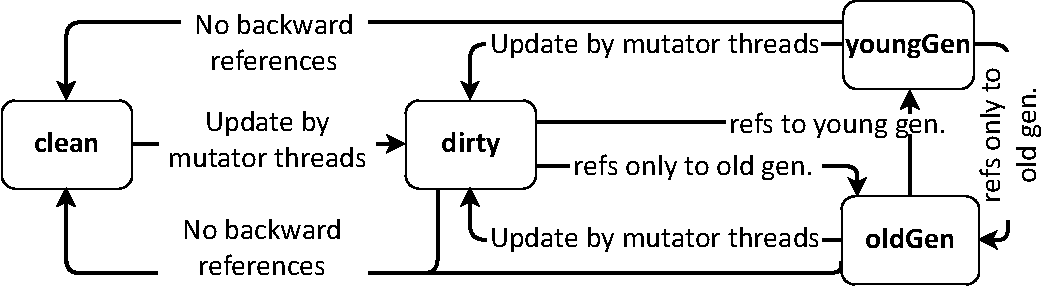
\includegraphics[width=0.5\linewidth]{teraheap/fig/h2_cards_state.pdf}}
  \hspace{10pt}
  \subfloat[]{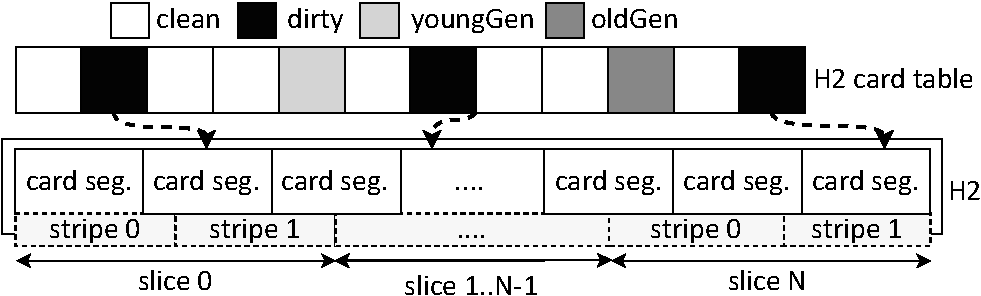
\includegraphics[width=0.45\linewidth]{teraheap/fig/h2_cardtable-crop.pdf}}
  \caption{(a) State transitions for H2 card
  table entries. (b) Organization of H2 as stripes and slices. }
\label{fig:h2cardtable}
\end{figure}

\paragraph{\textbf{Scanning H2 card table}}
\teraheapGC is multithreaded, and therefore, the H2 card table must support
concurrent accesses from multiple threads without synchronization.
Similar to H1, we divide H2 in slices and stripes to avoid contention
between \teraheapGC threads. As shown in Figure~\ref{fig:h2cardtable}(b), each
slice contains a number of fixed-size stripes equal to the number of
\teraheapGC threads. Each \teraheapGC thread operates on the stripes with the same id
in all H2 slices, avoiding thread contention.

In the native JVM, objects may span card segments and stripe
boundaries. Given that a separate \teraheapGC thread processes each stripe,
two threads may need to access each boundary (first and last) card in
a stripe. For this reason, the garbage collector avoids cleaning the
boundary cards in H1. If H1 boundary cards become dirty, they remain
dirty throughout execution. This phenomenon results in the garbage
collector scanning in every \teraheapGC the corresponding card segments for
objects with backward references.

This extra scanning would be significant drawback for H2 because (1) we use
large card segments to reduce H2 card table size and (2) the card segments are
mapped to a storage device, resulting in high I/O traffic when scanning objects.
\teraheapName{} resolves the issue of the dirty boundary cards by aligning objects to
stripes and guaranteeing that no two threads will need to access the same card.
\teraheapName{} uses stripe size equal to the H2 region size because \teraheapName{} guarantees
that objects do not span H2 regions.

